%%%%%%%%%%%%%%%%%%%%%%%%%%%%%%%%%%%%%%%%%%%%%%%
%%%     Declarations (skip to Begin Document, line 88, for parts you fill in)
%%%%%%%%%%%%%%%%%%%%%%%%%%%%%%%%%%%%%%%%%%%%%%%

%%\documentclass[10pt]{article}
%%\documentclass[10pt]{report}
%%\documentclass[letterpaper]{article}
\documentclass[12pt]{article}
\usepackage{geometry}
%\usepackage{xcolor}
\usepackage[table]{xcolor}
\usepackage{amsmath}
\usepackage[some]{background}
%\usepackage{lipsum}
%\usepackage{natbib}
\usepackage[utf8]{inputenc} % set input encoding to utf8

% V E R S I O N I N G
\usepackage{vhistory}

% U N I T S
%\usepackage[binary-units]{siunitx}
\usepackage[]{siunitx}

% L I N E  N U M B E R S
\usepackage{lineno}
%\linenumbers
 
% C I T A T I O N S
%\usepackage[backend=biber,style=apa]{biblatex}
\usepackage[backend=biber, style=apa, maxcitenames=1]{biblatex} 
%\DeclareLanguageMapping{english}{english-apa}
%\usepackage{apacite}
%\bibliographystyle{apa}

%\usepackage{biblatex} 
\addbibresource{paperpile.bib}
\usepackage{datetime}

%\usepackage{hyperref}

% Tables
\usepackage{float}
\usepackage[utf8]{inputenc}
\usepackage{tabularx}
\usepackage{booktabs}
\usepackage{longtable}

\usepackage{diagbox} %table split headers
\usepackage{longtable}
\usepackage{array}
\usepackage{rotating}
\usepackage{eqparbox}
\usepackage{makecell, caption, booktabs}
\usepackage{tablefootnote}

\usepackage{colortbl}

% Confusion Table
\usepackage{rotating}
\usepackage{xparse}
\usepackage{booktabs, makecell, multirow}
\NewExpandableDocumentCommand\mcc{O{1}m}
    {\multicolumn{#1}{c}{#2}}
\usepackage{siunitx}

% W A T E R M A R K 
% This gets rid of the draft watermark on the title page
\backgroundsetup{contents={}}
%\usepackage[text=DRAFT]{draftwatermark}

% L I N E  S P A C I N G
%\renewcommand{\baselinestretch}{1.5} 

% This does not have the effect I wanted, putting the caption at the bottom.
%\usepackage{caption}
%\captionsetup[table]{position=bottom} 

% Stuff needed to get table to span pages
\usepackage{enumitem}
%\usepackage{array, booktabs, longtable}
\newcolumntype{x}[1]{>{\raggedright}p{#1}}

\usepackage{etoolbox}
\AtBeginEnvironment{longtable}{%
    \setlist[itemize]{nosep,     % <-- new list setup
                      topsep     = 0pt       ,
                      partopsep  = 0pt       ,
                      leftmargin = *         ,
                      label      = $\bullet$ ,
                      before     = \vspace{-\baselineskip},
                      after      = \vspace{-0.5\baselineskip}
                        }
                           }% end of AtBeginEnvironment
% End table span

\definecolor{green}{rgb}{0.1,0.1,0.1}
%\color{green!40!yellow})

\newcommand{\done}{\cellcolor{teal}done}  %{0.9}
\newcommand{\hcyan}[1]{{\color{teal} #1}}

% Listings
\usepackage{listings}

\usepackage{geometry}  % Lots of layout options.  See http://en.wikibooks.org/wiki/LaTeX/Page_Layout
\geometry{letterpaper}  % ... or a4paper or a5paper or ... 
\usepackage{fullpage}  % somewhat standardized smaller margins (around an inch)
\usepackage{setspace}  % control line spacing in latex documents
\usepackage[parfill]{parskip}  % Activate to begin paragraphs with an empty line rather than an indent

\usepackage{amsmath,amssymb}  % latex math
\usepackage{empheq} % http://www.ctan.org/pkg/empheq
\usepackage{bm,upgreek}  % allows you to write bold greek letters (upper & lower case)

% for typsetting algorithm pseudocode see http://en.wikibooks.org/wiki/LaTeX/Algorithms_and_Pseudocode
\usepackage{algorithmic,algorithm}  

\usepackage{graphicx}  % inclusion of graphics; see: http://en.wikibooks.org/wiki/LaTeX/Importing_Graphics
% allow easy inclusion of .tif, .png graphics
\DeclareGraphicsRule{.tif}{png}{.png}{`convert #1 `dirname #1`/`basename #1 .tif`.png}

% \usepackage{subfigure}  % allows subfigures in figure
\usepackage{caption}
\usepackage{subcaption}

\usepackage{xspace}
\newcommand{\latex}{\LaTeX\xspace}

\usepackage{color}  % http://en.wikibooks.org/wiki/LaTeX/Colors

\long\def\todo#1{{\color{red}{\bf TODO: #1}}}

\long\def\ans#1{{\color{blue}{\em #1}}}
\long\def\ansnem#1{{\color{blue}#1}}
\long\def\boldred#1{{\color{red}{\bf #1}}}
\long\def\boldred#1{\textcolor{red}{\bf #1}}
\long\def\boldblue#1{\textcolor{blue}{\bf #1}}

% Useful package for syntax highlighting of specific code (such as python) -- see below
\usepackage{listings}  % http://en.wikibooks.org/wiki/LaTeX/Packages/Listings
\usepackage{textcomp}


%%% The following lines set up using the listings package
\renewcommand{\lstlistlistingname}{Code Listings}
\renewcommand{\lstlistingname}{Code Listing}

%%% Specific for python listings
\definecolor{gray}{gray}{0.5}
\definecolor{green}{rgb}{0,0.5,0}

\lstnewenvironment{python}[1][]{
\lstset{
language=python,
basicstyle=\footnotesize,  % could also use this -- a little larger \ttfamily\small\setstretch{1},
stringstyle=\color{red},
showstringspaces=false,
alsoletter={1234567890},
otherkeywords={\ , \}, \{},
keywordstyle=\color{blue},
emph={access,and,break,class,continue,def,del,elif ,else,%
except,exec,finally,for,from,global,if,import,in,i s,%
lambda,not,or,pass,print,raise,return,try,while},
emphstyle=\color{black}\bfseries,
emph={[2]True, False, None, self},
emphstyle=[2]\color{green},
emph={[3]from, import, as},
emphstyle=[3]\color{blue},
upquote=true,
morecomment=[s]{"""}{"""},
commentstyle=\color{gray}\slshape,
emph={[4]1, 2, 3, 4, 5, 6, 7, 8, 9, 0},
emphstyle=[4]\color{blue},
literate=*{:}{{\textcolor{blue}:}}{1}%
{=}{{\textcolor{blue}=}}{1}%
{-}{{\textcolor{blue}-}}{1}%
{+}{{\textcolor{blue}+}}{1}%
{*}{{\textcolor{blue}*}}{1}%
{!}{{\textcolor{blue}!}}{1}%
{(}{{\textcolor{blue}(}}{1}%
{)}{{\textcolor{blue})}}{1}%
{[}{{\textcolor{blue}[}}{1}%
{]}{{\textcolor{blue}]}}{1}%
{<}{{\textcolor{blue}<}}{1}%
{>}{{\textcolor{blue}>}}{1},%
%framexleftmargin=1mm, framextopmargin=1mm, frame=shadowbox, rulesepcolor=\color{blue},#1
framexleftmargin=1mm, framextopmargin=1mm, frame=single,#1
}}{}
%%% End python code listing definitions

\DeclareMathOperator{\diag}{diag}
\DeclareMathOperator{\cov}{cov}


%\bibliography{./paperpile.bib}
%\author{Evan McGinnis}
%\title{Automated Weeding}



\definecolor{titlepagecolor}{cmyk}{1,.60,0,.40}

\DeclareFixedFont{\bigsf}{T1}{phv}{b}{n}{1.5cm}

\backgroundsetup{
scale=1,
angle=0,
opacity=1,
contents={\begin{tikzpicture}[remember picture,overlay]
 \path [fill=titlepagecolor] (-0.5\paperwidth,5) rectangle (0.5\paperwidth,10);  
\end{tikzpicture}}
}
\makeatletter                       
\def\printauthor{%                  
    {\large \@author}}              
\makeatother
\author{%
\setstretch{1.0}
    Evan McGinnis \\
    PhD Student \\
    Student ID\#  23633780\\
    Biosystems Analytics \\
    \today \\
    \texttt{evanmc@arizona.edu}\vspace{40pt} \\
    }

\begin{document}

\begin{titlepage}
\BgThispage
\newgeometry{left=1cm,right=4cm}
\vspace*{1cm}
\noindent
%%\vspace*{0.4\textheight}
\textcolor{white}{\Huge\textbf{\textsf{Field Activities for Precision Treatment \\System for Weeds in Lettuce Crop}}}
\vspace*{2.5cm}\par
\noindent
\begin{minipage}{0.35\linewidth}
    \begin{flushright}
        \printauthor
    \end{flushright}
\end{minipage} \hspace{15pt}
%
\begin{minipage}{0.02\linewidth}
    \rule{1pt}{175pt}
\end{minipage} \hspace{-10pt}
%
\begin{minipage}{0.6\linewidth}
\vspace{5pt}
    \begin{abstract} 
\setstretch{1.0}
This paper details the field activities for the automated weeding project. While portions of this document repeat some details of the document referred to as \textit{the proposal}, this document assumes that readers are familiar with details covered there.
    \end{abstract}
\end{minipage}
\end{titlepage}
\restoregeometry
%
% F R O N T  M A T T E R
%
{
\setstretch{1.0}
\tableofcontents
\listoftables
\listoffigures
\newpage
}

{
\setstretch{1.0}
\begin{versionhistory}
  \vhEntry{1.0}{27 July 2022}{EM}{Initial revision}
\end{versionhistory}
\newpage
}


\section{Overview}
This phase will have two activities: installation of the physical hardware in the field enclosure, and field testing of the system. This phase will encompass these activities:
\begin{itemize}
	\item{Modify the existing enclosure and install components discussed in the proposal}
	\item{Field test the integrated system}
\end{itemize}
\subsection{Field Tests}
Field tests will be conducted at the Yuma Agricultural Center of the University of Arizona with the integrates system in two phases: data collection, and wet-runs. Prior to the execution of the data collection phase, however, two calibration activities will be carried out. Once executed, repeating this calibrations will not be required unless there there is a change in any physical equipment (this applies primarily to the vision and odometry subsystems).
\subsubsection{Sensor+Lens Calibration}
The objective of this phase is to determine the pixel to ground distance measurement when the weeding system is in a planting bed deemed 'typical'. This relationship is determined by the following steps\footnote{This calibration may not be required, as the relationship can be determined with some relatively simple equations. The ground sampling distance (GSD) will be $\approx$ \SI{0.02} {\centi\meter} per pixel, a figure that will not vary significantly even when the height of the planting bed varies by a few cm. As this figure far exceeds the precision of the emitter subsystem, it is not anticipated that even a small variation in this figure will have a negative impact on the system.}:
\begin{enumerate}
	\item{A calibration sheet with two green dots centered 4 cm apart is positioned directly beneath one camera}
	\item{Execute a script that will take the image, find the dots, determine the center-to-center distance in pixels. This script will write out a calibration file used by the weeding system}
\end{enumerate}
No forward motion of the weeding system will be required for this stage of the calibration. Calculations or laboratory tests to determine this relationship can be done, of course, but as the distance from the bed to the sensor will likely differ from measurements in the laboratory or used in calculations, this relationship will be determined by this field procedure.  A somewhat related procedure, but one that will be performed under laboratory conditions is the characterization of the distortion introduced by the lens in images of a checkerboard test target. A detailed description of that calibration is beyond the scope of this proposal, but is well documented elsewhere and supported by the OpenCV library set used for various imaging functions.
\subsubsection{Odometry Verification}
The odometry system will be verified on a level, hard, dry surface, under controlled (i.e., enclosed shed or equivalent) using this procedure:
\begin{enumerate}
	\item{A tape measure is placed on the ground along the cropline and extended the length of a planting bed.}
	\item{The weeding system is towed over the entire length at varying speeds including stops an backwards motion.}
\end{enumerate}
This test will compare actual ground distance to the values reported by the system.  As mentioned in Section~\ref{sec:odometry}, it is important that the odometry subsystem be accurate over the distance from the leading edge of the image captured to the emitter line, not accurate over the entire length of the planting bed.
\begin{figure}[H]
	\centering
	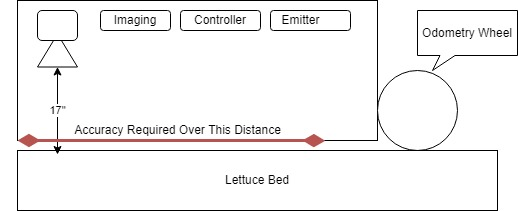
\includegraphics[width=0.75\linewidth]{./figures/odometry-accuracy.jpg}
	\caption[Accuracy required from odometry subsystem]{The odometery subsystem requires accuracy over only a portion of a planting bed, indicated by the red line in this diagram.  The accuracy over this distance must be +/- .5cm, twice the accuracy of the treatment subsystem.}
	\label{fig:uml-system}
\end{figure}
An odometry verification mode of the system software will capture and annotate images, noting every 1cm in forward motion to allow manual verification of accuracy.  Annotated images of the tape are used to verify two things:
\begin{enumerate}
	\item{Image capture accuracy --- Every increment on the tape should be captured, factoring in 20\% overlap at the leading and trailing edges of the image. To correctly classify vegetation that is not fully shown in a single image it will be necessary to stitch adjacent images together.}
	\item{Emitter distance accuracy --- The annotations in the images are not simply markers every 1cm. Rather, the image will be marked with the distance to the leading edge of the image captured by the odometry system.}
\end{enumerate}
\begin{figure}[H]
	\centering
	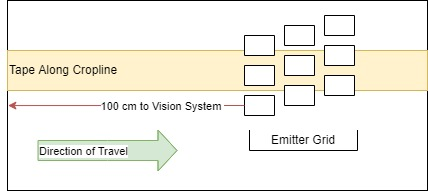
\includegraphics[width=0.75\linewidth]{./figures/test-distance.jpg}
	\caption[Test for distance measurement from emitter]{Note: not to scale. The distance from the center of the emitter to the leading edge of the image captured by the vision system. This figure uses a distance of 100cm only for illustration purposes. The value used will reflect distances in the physical system.}
	\label{fig:test-distance}
\end{figure}

While the absolute accuracy of this odometry system is calculated as noted by this equation:
\begin{align}
\frac {wheel\ circumference}  {rotational\ pulses},\  or\  \frac {92cm} {1000} = .092cm
\end{align}
annotating images with that sort of accuracy would result in too much visual clutter in the resulting image sets.

This procedure will be repeated under field conditions, where wheel slippage is expected to detrimentally affect accurate measurement of distance. Under both conditions, accuracy will be assessed both over the entire distance of a planting bed and over multiples of the distance shown above. These tests will not produce calibration data; their only purpose is to asses and adjust the odometry system.
\subsubsection{Data Collection}
While each run of the system will produce usable data, these "dry" runs will involve only the collection of speed, timing, classification, and imagery. There is no need for a complete and integrated treatment subsystem in these tests, but this phase must be preceded by the calibration tests detailed previously.
 In these runs, the system will collect a series of crop row images, each taken with 20\% front overlap. The image capture strategy reflects a need to stitch consecutive images together before classification, avoiding the problem where the lack of a full view of an object prevents classification. The images collected in this phase will be used for training in future runs, so runs early in this phase are unlikely to be acceptably accurate. Accuracy is expected to improve and will gate the transition to the next phase. Accuracy rates for phase exit will be 3\% false identification of crop as weeds, and 95\% correct identification of weeds as weeds.
The size of the each image set collected in this run will be dependent on several factors:
\begin{enumerate}
	\item{The size of the Region of Interest (ROI) --- the vision system proposed for this project (Basler) supports the notion of an ROI that may be a subset of the full capability of the sensor. Suppose that a strip above and below the crop line can be ignored. Capturing and processing this information may not be worthwhile.}
	\item{The compression rate of the camera system --- there is a tradeoff between image quality and the amount of compression applied. A 5 mega-pixel image contains 15 MB of data, but may be only 1 MB after compression. The image produced by the Basler acA1920-gc camera, for instance is 452 KB.}
	\item{The ground distance captured in each image}
	\item{The length of each planting bed row and the number of rows}
\end{enumerate}
Each image footprint is dependent on selections made for the vision subsystem. Using the values for a Basler acA1920-gc with a 5mm focal length lens\footnote{This camera was the only one available to the author at the time of this writing, and may not be chosen for the final project}, the image captured has these characteristics:
\begin{align}
	x = \left( \frac {elevation} {focal\ length} \right) \ *\ sensor\ width,\ or\ \left( \frac {502mm} {5mm} \right) 4.2mm = \SI{437.388}{\milli\meter} \\
	y = \left( \frac {elevation} {focal\ length} \right) \ *\ sensor\ height,\ or\ \left( \frac {502mm} {5mm} \right) 2.4mm = \SI{240.960}{\milli\meter}
\end{align}
The length of the planting bed and number of rows is variable, of course, but this proposal will assume there are four rows, each 20m in length. The total number of images is given by:
\begin{align}
	images = \frac {4 * 20m * \frac{1000mm} {1m}} {437.388mm * .8} = 228.63
\end{align}
The space needed for a single image capture set is:
\begin{align}
229\ images * \frac{\SI{452}{\kilo\byte}} {image} \approx \SI{103.5}{\mega\byte}
\end{align}

A \SI{64}{\giga\byte} flash drive on the Jetson will provide a minimum of \SI{40}{\giga\byte} of free space, enough for several image collections. It is not anticipated that this space will be used, however, as image sets will be automatically uploaded to CyVerse (for off-line analysis; this activity is not real-time) and deleted from local media upon the completion of a run and IP connectivity to CyVerse can be established.

\subsubsection{Wet-Run} 
This phase requires all subsystems to be functionally complete and integrated. During these runs, the identified weeds are treated with a tinted, non-toxic liquid.  Treatment efficacy and accuracy can be assessed in two ways:
\begin{enumerate}
	\item{Manually, by assessing the coverage of each plant by the treatment --- a manual assessment has the advantage of detailed inspection of each application, but suffers from the inevitable errors in any manual assessment.}
	\item{Automatically, by capturing images of post-treatment vegetation --- This approach would processes post-treatment images either by capturing images in real-time after treatment or by performing an additional dry-run immediately after a treatment, collecting an image set that can be used.  Collection of images immediately after treatment would require a new set of cameras immediately after the treatment system, a requirement that may not be mechanically feasible due to physical space constraints. The additional dry-run approach will be used in this project.}
\end{enumerate}
The automatic assessment of spray requires an image segmentation geared toward the hue of the dye, allowing the separation of treated vegetation. Once segmented, each unwanted plant is scored based on the percentage of leaf area treated. Once sufficient accuracy is achieved, treatment will transition from dyed water to dyed herbicide. Until that accuracy in achieved, weeds will be treated by manual remediation. Treatment accuracy should not be conflated with classification accuracy. While the classification of vegetation is an indication of the fate of a plant (treated or not, the intent), treatment accuracy is an indication of what actually happened. In practice, of course, the treatment accuracy will be 100\%, even if the classification is incorrect.


 \newpage
%
% W E A K N E S S E S
%
\section{Weaknesses of Study}
This proposal has weaknesses in four areas: weed/crop discrimination under field conditions, weed/crop discrimination over the growth cycle, system redundancy, and information security.

\subsection{Weed/Crop Discrimination Under Field Conditions}
While the concepts around this are explored in the proof of concept phase, the image sets used there are obtained under lighting conditions that will  not be encountered in the production phase. The structural features noted previously will probably be invariant to changes based on lighting -- how round an object is does not depend heavily on lighting conditions, for instance. Color features, however, may. Vegetation may exhibit different responses to LED light than to full-spectrum sunlight. If this is encountered, we plan to deal with this by either adjusting the aforementioned thresholds applied to a vegetation index, or to use an index more suited to the spectrum encountered.

%\subsection{Weed/Crop Discrimination over the Grown Cycle}

\subsection{Redundancy}
The system described in this proposal has multiple single points of failure. In such a system, for instance, the failure of a shared resource -- such as the National Instruments RIO controller -- would render the entire system unusable. The failure of a resource dedicated to a task, but with a peer performing the same task -- such as processing the images along the right side of a row -- will result in the degradation of system, but not a complete failure.
\begin{figure}[H]
	\centering
	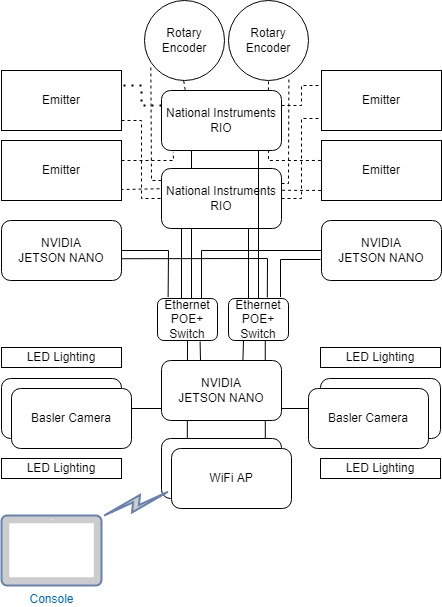
\includegraphics[width=0.4\linewidth]{./figures/system-overview-Page-2.jpg}
	\caption[An overview of a redundant system]{An overview of a redundant system, illustrating that there is no single point of failure}
	\label{fig:system-overview-redundant}
\end{figure}

Figure~\ref{fig:system-overview-redundant} illustrates a system without a single point of failure. If a RIO controller fails, for example, the system can use the redundant controller. If an Ethernet switch fails or if a cable fails connecting a component, that component can use the redundant network. In these systems, there are redundancy decisions that can be made locally -- a link to a switch has failed and the other switch must be used --- and redundancy decisions that must be made system-wide -- the failure of a component hosting the messaging server, for instance. That the system shows three NVIDIA devices is indicative of the N+1 redundancy scheme used by such a system. This system can tolerate the loss of only one NVIDIA, as it must have a \textit{quorum} of members to form a redundancy group. It is beyond the scope of this proposal to discuss redundancy schemes in depth, and the overly broad statements here are not meant to be an analysis of failure scenarios. \\
For the proposed system, we will characterize the risk by computing MTBF of the physical components (these may not be available for components, but are typically supplied by the vendor).  While it does not mitigate the risk, system components will perform extensive self-tests when the system is first brought up, as well as non-invasive self tests during system operation. These self test results will speed the identification of faulty components, leading to higher uptimes and simplifying field deployments.
 
\subsection{Information Security}
This proposal does not address the information security of the system, and a full assessment of that topic is beyond the scope of this document. While this system does not control a high-value target, the opportunities for compromising the subsystems can not be ignored entirely. The final system will take some best-practices approach to system components:
\begin{itemize}
	\item{Minimize the attack surface by shutting down unneeded services}
	\item{Using certificates in lieu of passwords for establishing communication}
	\item{Encrypting all communications between components}
	\item{Scanning the system with penetration testing software}
\end{itemize}


%\newpage
%\section{Public Health Significance}
 
%\section{Budget}
%\label{section:budget}
%Table~\ref{table:budget} reflects the total expenditures involved in this study. While not broken down by year, it is anticipated that these expenditures will take place over two years. Amounts specified are in US\$.
%\begin{table}[h]
%\centering
%\begin{tabular}{lrlr}
% 	\toprule
%	Salaries/Wages    &  & 2670.60 \\
%	\midrule
%	& Mechanicals & 1965.00 \\
%	&Field Operator & 705.60 \\
%	\midrule
%	Travel & & 2241.72 \\
%	\midrule
%	& In State & 2241.72 \\
%	\midrule
%	Supplies & & 6789.00 \\
%	\midrule
%	\midrule
%	Project subtotal & & 11701.32 \\
%	\midrule
%	Indirect Costs (53\%)\tablefootnote{This may not be required if separate funding is not obtained. If that is not the case, the project subtotal should be considered the grand total for the project.} & & 6201.70 \\
%	\toprule
%	\toprule
%	\textsc{Total Project}                      & & \underline{18387.92} \\
%
%	\bottomrule
%    \bottomrule                
%\end{tabular}
%\caption[Total Budget Breakdown]{A breakdown of expenditures for this study}
%\label{table:budget}
%\end{table}
%
%%
%% S A L A R I E S
%%
%\subsection{Salaries and Wages}
%Table~\ref{table:salaries} reflects the salary expenditures for this study.  The components discussed in Section~\ref{section:system} will need to be installed in the existing enclosure. To accommodate these components, mechanical modifications will be required and will be carried out at the Yuma Agricultural Research Center. Once a modified system is ready, an operator qualified to operate a tractor in a field setting will conduct test runs using the system at the Valley Farm site of the Yuma Agricultural Research center.
%\begin{table}[H] % Force the table to show below the paragraph
%\centering
%\begin{tabular}{lrlrlrlrlrlrlr}
% 	\toprule
%	Role & Per Hour & Hours Per Week & Weeks & ERE & Subtotal \\
%	\toprule
%	Mechanicals & 25.00 & 20 & 3 & 31.0\% & 1965.00 \\
%	Field Operator & 15.00 & 2 & 20 & 17.6\% & 705.60 \\
%	\toprule
%	\toprule
%	\textsc{Total Salaries} & & & & & \underline{2670.60} \\
%
%	\bottomrule
%    \bottomrule                
%\end{tabular}
%\caption[Salary Breakdown]{A breakdown of salaries for this study}
%\label{table:salaries}
%\end{table}
%
%%
%% T R A V E L
%%
%
%\subsection{Travel}
%Travel funds dedicated for in-state travel represent 6 trips to Yuma, Arizona to oversee physical system integration of the automated system and to oversee and collect data from field trials. These activities both take place at the University of Arizona Yuma Agricultural Center.
%\begin{table}[H] % Force the table to show below the paragraph
%\centering
%\begin{tabular}{lrlr}
% 	\toprule
%	\toprule
%	6 Trips to Yuma, AZ & & 2241.72 \\
%	\midrule
%	& Vehicle Rental for 2 days per trip @ \$67.31 & 1407.72 \\
%	& Lodging for 1 day per trip @ \$94.00 & 564.00 \\
%	& M\&IE for 2 days per trip @ \$45.00 & 270.00 \\
%	\toprule
%	\toprule
%	\textsc{Total Travel}                      & & \underline{2241.72} \\
%	\bottomrule
%    \bottomrule                
%\end{tabular}
%\caption[Travel Budget Breakdown]{A breakdown of travel expenditures for this study}
%\label{table:travel}
%\end{table}

%
% S U P P L I E S
%
\section{Supplies}
\label{section:supplies}
Table~\ref{table:supplies} reflects the supply expenditures for this proposal. All of the supplies here represent the Bill of Materials (BOM) of the final system, and will be installed in the existing enclosure. These supplies are required to support the completion of the \textit{deployment} phase detailed in Section~\ref{section:phases}.\\

\begin{table}[H] % Force the table to show below the paragraph
\centering
\begin{tabular}{lrlr}
 	\toprule
 	Item & Quantity & Price \\
 	\midrule
	Heavy Duty TRD-GK Rotary Encoder & 1 & 269.00 \\
	NVIDIA Jetson & 2 @ 459 &918.00 \\
	NVIDIA Jetson Enclosure &2 @ 25 & 50.00 \\
	LED Lamps & 4 @ 150 & 600.00 \\
	National Instruments CompactRIO&1& 1567.00 \\
	9411 Module for RIO &1& 372.00 \\
	9403 Module for RIO &1& 656.00 \\
	Cables &6+& 75.00 \\
	Basler ACE2 Machine Vision Camera &2 @ 730& 1460.00  \\
	Computar C-Mount Lens &2 @ 320& 640.00 \\
	POE+ Ethernet Switch &1& 50.00 \\
	WiFi Outdoor Access Point &1& 70.00 \\
	Encoder Power Supply &1& 12.00 \\
	NVIDIA Jetson Power Supply &2 @ 25& 50.00 \\
	\midrule
	\midrule
	\textsc{Total Supplies}                      & & \underline{6789.00} \\
	\bottomrule
    \bottomrule                
\end{tabular}
\caption[Supply Budget Breakdown]{A breakdown of supply expenditures for the deployment stage of this study}
\label{table:supplies}
\end{table}




%\end{table}

%REFERENCES
%Use the Vancouver Style of referencing. This is found at this website:
%http://www.ncbi.nlm.nih.gov/books/bv.fcgi?rid=citmed.TOC&depth=2 or a less detailed website:
%http://www.nlm.nih.gov/bsd/uniform_requirements.html
%
%References should be numbered consecutively in the order in which they are first mentioned in the text. Identify references in text, tables, and legends by Arabic numerals in parentheses. The titles of journals should be abbreviated according to the style used in Index Medicus. Consult the list of Journals Indexed for MEDLINE, published annually as a separate publication by the National Library of Medicine. The list can also be obtained through the Library's web site..



 


% 
% E N D  T E M P L A T E  F R O M  W O R D
%

\newpage
{
\setstretch{1.0}
\section{References}
\printbibliography[heading=none]
}

\end{document}

